\documentclass[tikz,border=0pt]{standalone}
\usepackage[utf8]{inputenc}
\usepackage{csquotes}
\usepackage{xcolor}
\usepackage{graphicx}
\usepackage{pgffor}
\usepackage{listings}
\usepackage{array}
\usepackage{fontawesome}
\usepackage{amsmath}

\lstset{
    basicstyle=\ttfamily\fontsize{6}{8}\selectfont,
    breaklines=true,
    % backgroundcolor=\color{black},
    keywordstyle=\color{pink},
    commentstyle=\color{blue},
    stringstyle=\color{white},
    showstringspaces=false,
    frame=none,
    xleftmargin=0.6cm,
    xrightmargin=0.6cm
}

\begin{document}
\begin{tikzpicture}
\useasboundingbox (0,0) rectangle (10.8,10.8);

% Hintergrund in Schwarz
\fill[black] (0,0) rectangle (10.8,10.8);

% Zufällige Einsen und Nullen verteilen
\foreach \i in {1,...,5000} {
    \node[text=green, opacity=0.1, font=\ttfamily\fontsize{5}{6}\selectfont] at (rand*10.8, rand*10.8) {\pgfmathtruncatemacro{\random}{round(rand)}\random};
}

% \fill[red, opacity=0.1] (0.05,5.95) rectangle (10.75,10.75);
% \draw[red, thin] (0.05,5.95) rectangle (10.75,10.75); % 45% Höhe
\node[red, anchor=north west, font=\ttfamily\bfseries\fontsize{8}{9}\selectfont] at (0.1,10.65) {NVD DB Update {\Large{ CVE-2025-20634} - \textbf{Score:}{\Large{ 9.8 }}}};
% % ------------------------------------------------------------------------------------------------------------------------------
% \node[red, anchor=north west, font=\ttfamily\fontsize{8}{9}\selectfont, text width=10.6cm, align=center] at (0.1,10.25) {
% \newline
% \newline
% \newline
% If you want to succeed in penetration testing and cybersecurity, learn at least:
% \newline
% };
% ------------------------------------------------------------------------------------------------------------------------------
\fill[green, opacity=0.1] (0.05,1.15) rectangle (10.75,10.75);
\draw[green, thin] (0.05,1.15) rectangle (10.75,10.75); % 45% Höhe
% \node[green, anchor=north west, font=\ttfamily\bfseries\fontsize{8}{9}\selectfont] at (0.1,5.65) {Solution:};
% ------------------------------------------------------------------------------------------------------------------------------
\node[green, anchor=north west, font=\ttfamily\fontsize{8}{9}\selectfont, text width=10.6cm, align=center] at (0.1,10.25) {
\textbf{Components:}
\begin{scriptsize}
\begin{lstlisting}
 mediatek mt6983 -
 mediatek mt6980 -
 mediatek mt2737 -
 mediatek mt6895tt -
 mediatek mt6835 -
 mediatek mt6896 -
 mediatek mt6895 -
 mediatek mt6886 -
 mediatek mt6813 -
 mediatek mt6897 -
 mediatek mt6878 -
 mediatek mt6899 -
 mediatek mt6835t -
 mediatek mt6879 -
 mediatek mt6980d -
 mediatek nr16 -
 mediatek nr17 -
 mediatek nr17r -
 mediatek mt6878m -
\end{lstlisting}
\end{scriptsize}
\textbf{Description:}
\begin{scriptsize}
\begin{lstlisting}
In Modem, there is a possible out of bounds write due to a missing bounds check. This could lead to remote code execution, if a UE has connected to a rogue base station controlled by the attacker, with no additional execution privileges needed. User interaction is not needed for exploitation. Patch ID: MOLY01289384; Issue ID: MSV-2436.
\end{lstlisting}
\end{scriptsize}
\textbf{Main problems:}
\begin{scriptsize}
\begin{lstlisting}
787 "Out-of-bounds Write"

\end{lstlisting}
\end{scriptsize}
};
% ------------------------------------------------------------------------------------------------------------------------------
\draw[green, thin] (0.05,0.05) rectangle (10.75,1.05); % 10% Höhe
% \node[green, anchor=north west, font=\ttfamily\bfseries\fontsize{5}{6}\selectfont] at (0.1,0.95) {Contact:};

% Tabelle 2x2 im Contact Block
\node[green, anchor=north west, font=\ttfamily\fontsize{8}{9}\selectfont, text width=10.6cm] at (0.1,0.95) {
\begin{tabular}{@{}p{4.8cm}@{}p{5cm}@{}}
\faGlobe\ https://cybersword.tech & \faLinkedin\ www.linkedin.com/in/cybersword-tech \\
\faInstagram\ ph1sher & \faTwitter\ @davidwowa \\
\end{tabular}
};
\end{tikzpicture}
\end{document}